\documentclass[a4paper]{article}

% Basic packages
\usepackage[fontset=fandol]{ctex}
\usepackage{amsmath, amssymb}
\usepackage{graphicx}
\usepackage[margin=2.5cm]{geometry}
\usepackage[most]{tcolorbox}
\usepackage{etoolbox}
\usepackage{listings}
\usepackage{hyperref}
\usepackage{booktabs}
\usepackage{subcaption}
\usepackage{float}
\usepackage{tikz}
\IfFileExists{pgfplots.sty}{
    \usepackage{pgfplots}
    \pgfplotsset{compat=1.18}
}{}

% Highlight boxes
\newtcolorbox{knowledgebox}[1]{
    enhanced, colback=blue!5!white, colframe=blue!75!black, colbacktitle=blue!75!black,
    coltitle=white, fonttitle=\bfseries, title=#1, attach boxed title to top left={yshift=-2mm, xshift=2mm},
    boxrule=1pt, sharp corners
}

\newtcolorbox{importantbox}[1]{
    enhanced, colback=yellow!10!white, colframe=yellow!80!black, colbacktitle=yellow!80!black,
    coltitle=black, fonttitle=\bfseries, title=#1, sharp corners
}

\newtcolorbox{warningbox}[1]{
    enhanced, colback=red!5!white, colframe=red!75!black, colbacktitle=red!75!black,
    coltitle=white, fonttitle=\bfseries, title=#1, sharp corners
}

% Listings
\lstset{
    language=Python,
    basicstyle=\ttfamily\small,
    keywordstyle=\color{blue},
    stringstyle=\color{red!60!black},
    commentstyle=\color{green!60!black},
    breaklines=true,
    frame=single,
    numbers=left,
    numberstyle=\tiny\color{gray},
    captionpos=b,
    extendedchars=false
}

% Front-page metadata
\newcommand{\notetitle}{CS336 第 14 讲：数据工程 II}
\newcommand{\noteauthors}{Codex 基于 Stanford CS336 2025 第 14 讲视频、字幕与课程材料整理}
\newcommand{\notedate}{\today}
\newcommand{\videochannel}{Stanford Online}
\newcommand{\videopublishdate}{2025年06月16日}
\newcommand{\videoduration}{1:19:11}
\newcommand{\videourl}{https://www.youtube.com/watch?v=9Cd0THLS1t0}
\newcommand{\videocoverpath}{cover.jpg}

\begin{document}

\begin{titlepage}
\centering
{\Large 课程笔记\par}
\vspace{1.2cm}
{\huge\bfseries \notetitle\par}
\vspace{0.8cm}
{\large \noteauthors\par}
\vspace{0.3cm}
{\large \notedate\par}
\vspace{1.2cm}

\ifdefempty{\videocoverpath}{
{\small 请在生成笔记时填入视频封面图的本地路径。\par}
}{
\includegraphics[width=0.82\textwidth,height=0.45\textheight,keepaspectratio]{\videocoverpath}\par
}

\vfill
\begin{tcolorbox}[width=0.9\textwidth, colback=black!2!white, colframe=black!60, sharp corners]
\textbf{视频作者/频道}：\videochannel\par
\textbf{发布日期}：\videopublishdate\par
\textbf{视频时长}：\videoduration\par
\textbf{视频链接}：
\ifdefempty{\videourl}{
未填写
}{
\href{\videourl}{\nolinkurl{\videourl}}
}
\end{tcolorbox}
\end{titlepage}

\tableofcontents
\newpage

%% --- 正文内容开始 --- %%

\section{Data II：从“知道数据重要”到“真的会筛、会选、会去重”}

\subsection{课程为什么要单独讲算法工具}
第 13 讲是全景图，告诉你数据是能力护城河；第 14 讲则开始拆机械结构：如果你手里有一大池原始数据 $R$，再给你一小份“你真正想要的”目标数据 $T$，怎样从 $R$ 中找出一个更像 $T$ 的子集 $T'$？

这就是课程设定的统一抽象。它之所以重要，是因为很多数据工程任务都能被写成这个模式：想找英文文本、想找高质量教育文本、想找数学文本、想去掉有毒或重复内容，本质上都是在巨大的原始候选池里做选择，而不是凭空造数据。

\begin{figure}[H]
\centering
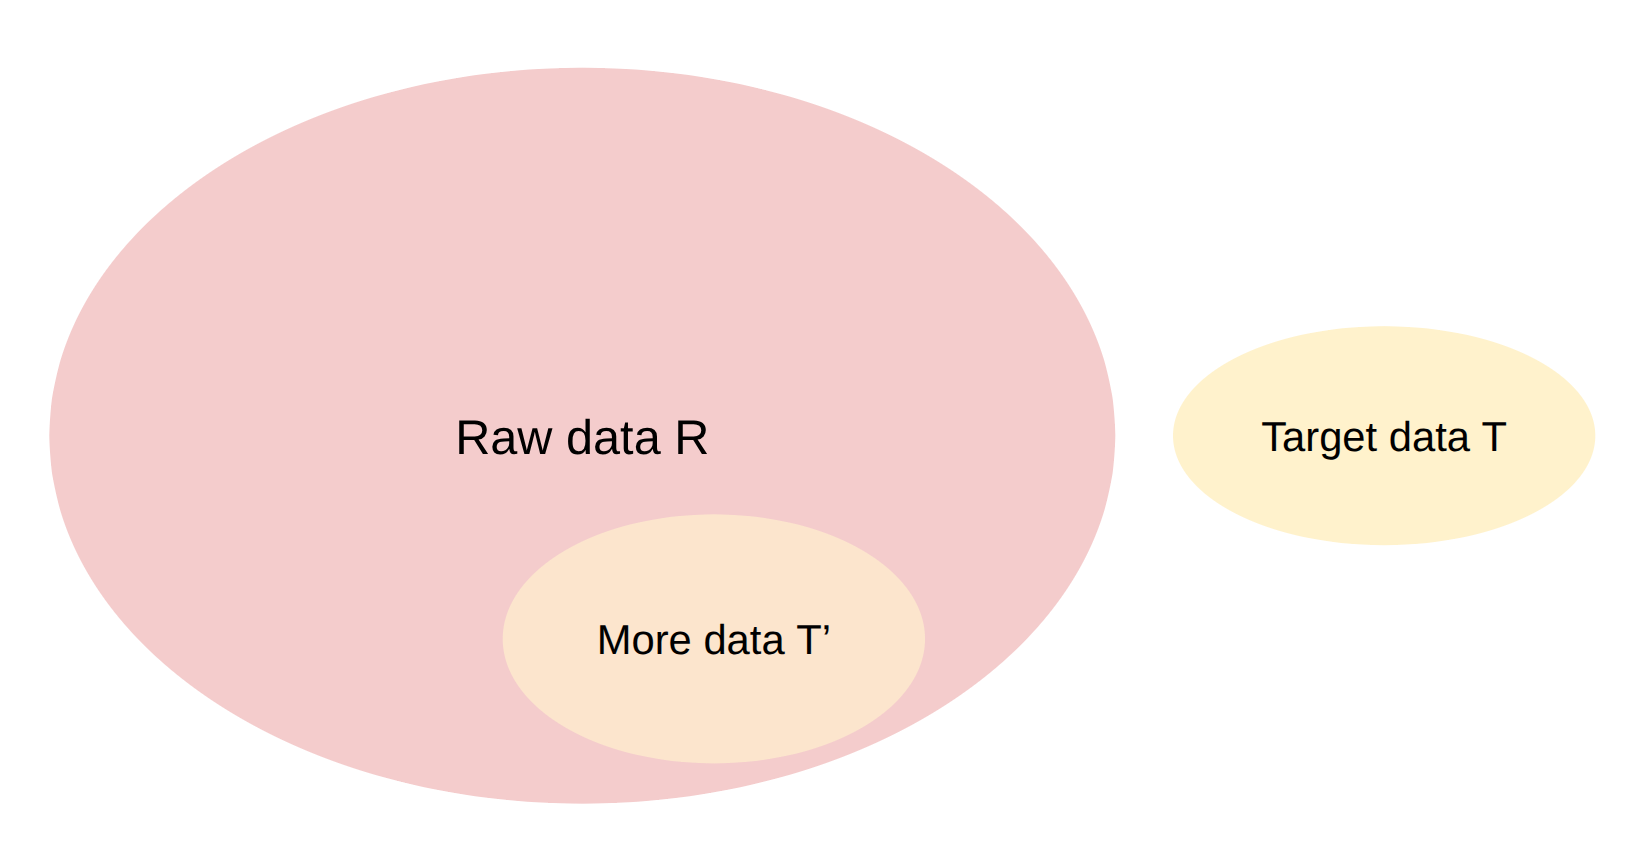
\includegraphics[width=0.78\textwidth]{../../materials/spring2025-lectures/images/raw-target-schema.png}
\caption{课程用一个统一的 schema 描述数据选择问题：从巨大的 raw pool 中挑出更接近目标分布的子集。}
\end{figure}

\begin{importantbox}{第 14 讲的总目标}
把“数据质量很重要”这句正确但空泛的话，具体化成一套可以在线性规模上运行的算法工具：语言模型打分、线性分类器、重要性重采样、哈希去重与近重复检测。
\end{importantbox}

\subsection{本章小结}
第 14 讲首先把数据处理抽象成“目标分布选择”问题。只要抓住这个统一视角，后面的 KenLM、fastText、DSIR 和 MinHash 就不再是零散技巧，而是同一类问题的不同解法。

\section{KenLM 与 CCNet：用 n-gram 语言模型做快速质量过滤}

\subsection{为什么课程先讲最简单的模型}
课程没有一上来就用大型神经网络做过滤，而是先讲 n-gram 语言模型和 KenLM。这很有深意，因为数据工程的第一约束常常不是“模型够不够强”，而是“你能不能在海量语料上跑得动”。KenLM 这类方法虽然粗糙，却极快，因此非常适合做第一层筛选。

对一个 $n$-gram 语言模型，最基本的极大似然估计可以写成：
\[
p(w_t \mid w_{t-n+1:t-1}) = \frac{\mathrm{count}(w_{t-n+1}, \ldots, w_t)}{\mathrm{count}(w_{t-n+1}, \ldots, w_{t-1})}.
\]
课程马上提醒，真实语料里高阶 $n$-gram 非常稀疏，所以必须做 Kneser-Ney smoothing 之类的平滑。直观上，这就是在说：如果长上下文统计不可靠，就适度退回更短上下文。

\subsection{CCNet 的关键思想：保留“看起来像高质量语料”的文档}
CCNet 的做法很有代表性。它把段落或文档放进一个简单语言模型里，根据 perplexity 或近似分数排序，再保留更像目标高质量文本的那一部分。课程拿它来说明一个很有力量的观点：\textbf{“好数据”并不一定要靠昂贵模型判断，很多时候一个高速但粗糙的打分器就能显著改善训练语料。}

这种方法的优势是速度快、易扩展、可用于低资源语言；缺点也很明显，它只能抓住非常粗粒度的语言分布相似性，难以表达更抽象的“教育性”“事实性”或“任务价值”。

\begin{knowledgebox}{KenLM 的真正定位}
课程并没有把 KenLM 当成终极方案，而是当成“在海量语料上先做一轮粗筛”的基础工具。它便宜、可扩展、足够解释性强，因此很适合做 pipeline 里的第一层。
\end{knowledgebox}

\subsection{本章小结}
KenLM 和 CCNet 代表了一类朴素但高性价比的数据工程方法：先用可扩展的语言模型近似“目标文档长什么样”，再按分数做快速筛选。

\section{fastText 与 DSIR：从分类到分布匹配}

\subsection{fastText：用线性分类器学“什么像目标数据”}
课程接着讲 fastText，核心原因仍然是它快。fastText 本质上是带词嵌入平均和哈希 n-gram 的线性分类器，训练和推理都远比大型 Transformer 轻量。对于“英语还是非英语”“高质量还是低质量”“有毒还是无毒”这类二分类任务，它往往已经够用。

课程的重点不是 fastText 的每个细节，而是它提供了一种从启发式规则升级到学习式过滤的桥梁：不再手写“哪些词像垃圾”，而是收集正负样本，训练一个分类器，然后把它跑到整个数据池上。这种思路在语言识别、质量过滤、毒性过滤里都反复出现。

\subsection{为什么 fastText 比朴素 bag-of-words 更适合海量语料}
课程这里其实隐含了一层重要的参数化直觉。最朴素的 bag-of-words 分类器，如果词表大小是 $V$、类别数是 $K$，直接做线性分类往往需要大约 $V\times K$ 个参数。对于超大词表和多语言场景，这个参数量会非常难看。

fastText 的思路是先给词学习一个低维向量，再把文档中的词向量做平均或求和，于是参数规模更接近
\[
H(V+K),
\]
其中：
\begin{itemize}
\item $V$：词表大小；
\item $K$：类别数；
\item $H$：嵌入维度。
\end{itemize}

这比直接给每个词、每个类别都配一套独立权重更省，也让并行 SGD 和流式训练更现实。课程随后又补了一步：当我们把 bigram、trigram 也纳入特征时，特征空间会爆炸，于是需要 hashing trick 把这些 n-gram 映射到固定桶里。也就是说，\textbf{fastText 好用不只是因为“它是线性模型”，而是因为它把参数规模和特征规模都压进了一个能在网页语料上跑起来的范围。}

\subsection{DSIR：不只看像不像目标，还看原始分布有多不同}
比分类器更进一步的是 DSIR（Data Selection via Importance Resampling）。课程把它解释成一个更“分布论”的做法：你不只是判断某个样本是不是目标类，而是想估计它在目标分布 $p_T$ 下比在原始分布 $p_R$ 下有多“值得被保留”。

它的核心分数可以写成：
\[
s(x) = \frac{p_T(x)}{p_R(x)}.
\]
如果某个样本在目标分布下相对更常见、在原始分布下相对没那么常见，那么这个样本就更值得被重采样进新语料。课程用 DSIR 想说明：\textbf{数据选择不一定只是二分类，也可以是更细腻的分布重加权问题。}

\begin{figure}[H]
\centering
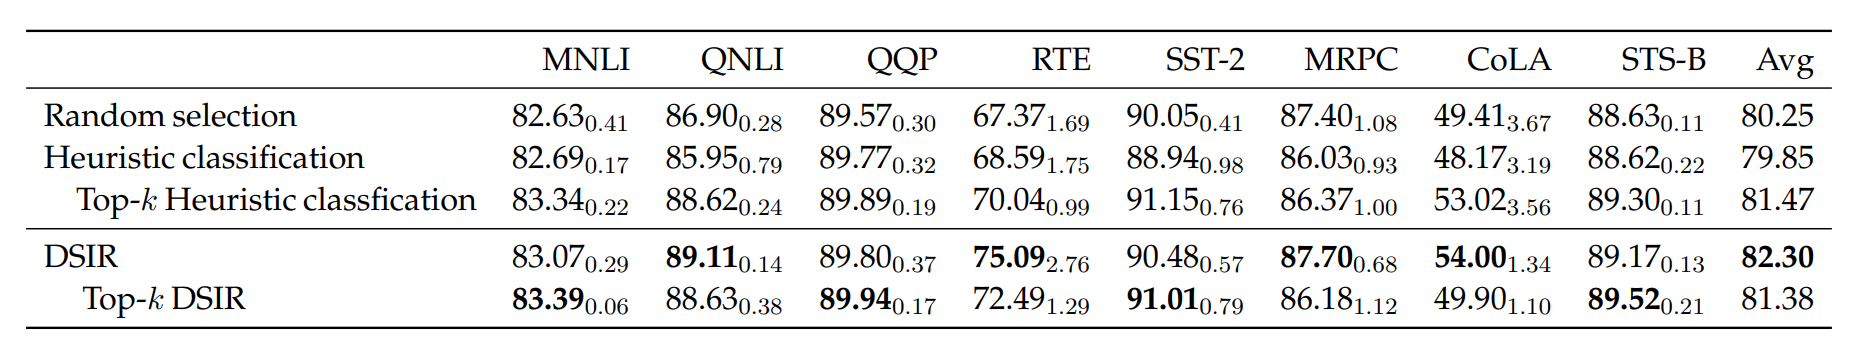
\includegraphics[width=0.82\textwidth]{../../materials/spring2025-lectures/images/dsir-results.png}
\caption{DSIR 通过重要性重采样，有时能比启发式分类拿到更好的下游效果。}
\end{figure}

\subsection{为什么课程把 fastText 和 DSIR 放在一起讲}
因为二者代表了两种不同层次的建模方式。fastText 更像判别式分类器，学的是“像不像目标”；DSIR 更像概率比估计，学的是“这个样本相对来说更应该来自哪个分布”。它们计算复杂度相近，但表达的统计假设不同。

\begin{warningbox}{关于“更智能的数据选择”的一个现实提醒}
方法越复杂，不代表一定越好。课程强调，真正的约束来自规模和可部署性。一个理论上更漂亮但跑不动的选择器，在 240T token 语料面前往往毫无价值。
\end{warningbox}

\subsection{从 OpenMathText 到 phi-1：target 定义决定过滤器会偏向什么}
课程随后举了几类非常有代表性的应用。OpenMathText 用规则加 KenLM、fastText 去找“更像数学文本”的网页；GPT-3 和 LLaMA 这类工作会把 Wikipedia、WebText 或参考页面当作正例，学“更像优质网页”的过滤器；phi-1 则更激进，直接围绕“高质量教材风格代码数据”去选样本。

这些案例背后有同一个结论：过滤器从来不是抽象地学“好数据”，而是在学“更像哪一种好数据”。如果你的正例偏向百科和书面文风，模型就会被拉向那一侧；如果正例偏向教育性解释或数学证明，模型就会在那些能力上更容易占便宜。课程把这些例子放在一起，其实是在提醒学生：\textbf{数据选择算法只是一半，另一半是你拿什么来定义目标分布。}

\subsection{本章小结}
fastText 和 DSIR 把数据工程从“规则过滤”推进到了“学习式选择”。前者擅长快速分类，后者擅长分布重加权，二者一起构成了现代过滤 pipeline 的主干。

\section{同一套工具可以服务很多任务：语言识别、质量过滤、毒性控制}

\subsection{课程为什么强调“先统一框架，再谈应用”}
第 14 讲很强调一个思想：同样的数据选择 machinery 可以复用于不同任务。只要你能定义目标数据 $T$，就可以把语言识别、数学文本筛选、教育价值筛选和毒性过滤都放进同一个框架里。

例如语言识别可以用 off-the-shelf 的 fastText 语言分类器；质量过滤可以让目标语料来自 Wikipedia、WebText 或高质量 instruction data；毒性过滤则可以把 Jigsaw 一类带标注的评论数据当作监督源。差别不在算法骨架，而在你选了什么 target，以及阈值设在哪里。

\subsection{目标定义本身就是价值判断}
课程在这里的启发很强。所谓“高质量数据”并不是自然存在的，而是由你选取的正负样本定义出来的。如果你拿 OpenHermes、ELI5 做正例，你学出来的是一种偏教育性、解释性、任务导向的 quality prior；如果你拿 Wikipedia references 做正例，你学出来的就是另一种 prior。

这意味着数据工程并不是中立流水线。选择什么目标，实际上就是在决定模型以后更擅长什么风格、什么语域和什么任务。

\subsection{本章小结}
同一个算法框架可以被重复利用，但目标定义永远不是中性的。课程借此提醒学生：数据筛选同时是在做价值选择。

\section{去重不是附属工作，而是线性规模训练的必要条件}

\subsection{为什么重复数据会系统性伤害训练}
课程在去重部分首先说明了为什么这件事如此重要。重复文本会带来两类问题：第一，浪费 token 预算，让模型反复在同样内容上优化；第二，增加记忆化风险，放大版权和隐私问题。特别是在网页、代码和论坛数据中，镜像、模板、fork、转载和轻微改写都极其常见。

因此，去重不是“锦上添花”的清洗步骤，而是大规模训练能否有效利用算力的前提条件。

\subsection{从 exact duplicates 到 near duplicates}
课程把重复分成 exact duplicates 和 near duplicates。exact match 可以直接哈希后去重，语义很清晰；但大量现实重复并不是逐字相同，而是只差几个 token、几个段落或格式细节。于是我们需要一个更弱但更可扩展的相似性定义。

课程采用的标准度量是 Jaccard 相似度：
\[
J(A, B) = \frac{|A \cap B|}{|A \cup B|}.
\]
如果把文档表示成 n-gram 集合，那么 Jaccard 就能自然描述两个文档共享多少局部内容。

\begin{figure}[H]
\centering
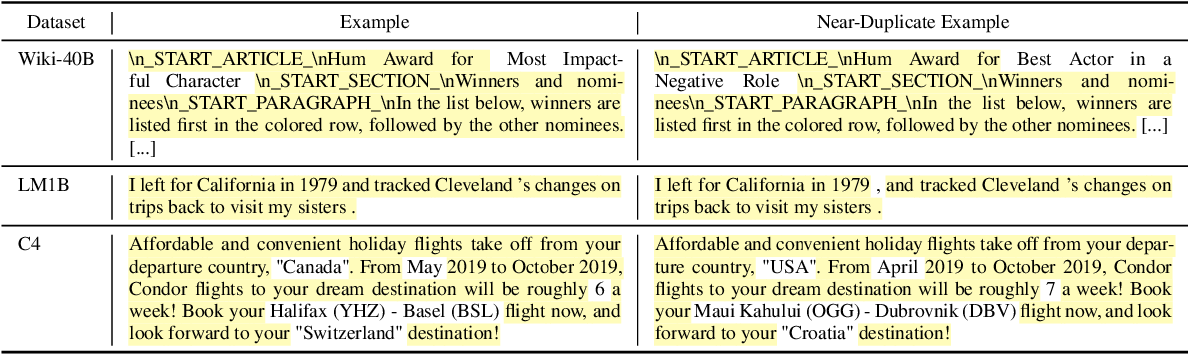
\includegraphics[width=0.9\textwidth]{near_duplicate_examples.png}
\caption{课程给出的 near-duplicate 例子：文字表面不同，但大量局部 n-gram 几乎完全重合。}
\end{figure}

\subsection{Bloom filter、MinHash 与 LSH 为什么能在线性时间里工作}
课程非常强调可扩展性。Bloom filter 提供的是近似集合成员测试，用很小内存换取极低误判率；MinHash 的关键性质是：
\[
\Pr[h(A)=h(B)] = J(A, B),
\]
也就是说，哈希碰撞概率直接等于 Jaccard 相似度。再往上，通过 locality-sensitive hashing（LSH）把多个 MinHash 按 band 组织起来，就能把“相似文档更容易碰撞”变成“超过阈值的文档几乎一定被提名”。

课程虽然没有要求学生记住所有推导细节，但它明确给出一个高度值得记住的式子：如果单个 band 有 $r$ 个哈希，总共 $b$ 个 band，相似度为 $s$ 的两个样本被提名为候选的概率近似是
\[
1 - (1 - s^r)^b.
\]
这说明 banding 结构可以把原本平滑的碰撞概率，压成一个更接近阈值函数的选择器。

\subsection{Bloom filter 是去重流水线里的低成本门卫}
课程在 MinHash 之前先讲 Bloom filter，不是因为它更“高级”，而是因为它在 exact duplicate 和近似成员测试上都太实用了。Bloom filter 的核心是：用 $k$ 个哈希函数把一个元素映射到一个位数组里，只要某一位为 0，就能确定该元素不在集合中；如果对应位都为 1，它“很可能”在集合中，但也可能是误判。

在常见近似下，Bloom filter 的假阳性率可以写成
\[
f \approx \left(1 - e^{-kn/m}\right)^k,
\]
其中：
\begin{itemize}
\item $n$：插入元素数；
\item $m$：位数组大小；
\item $k$：哈希函数数量；
\item $f$：假阳性概率。
\end{itemize}

课程想让学生看到的是一个典型工程权衡：更多内存 $m$ 会降低误判，更多哈希函数 $k$ 也会降低误判，但会增加计算量。最优 $k$ 大约在
\[
k^\star \approx \frac{m}{n}\ln 2
\]
附近。像 Dolma 这样的数据集之所以能把 paragraph 级去重推到极低误判率，就是因为它愿意在这一步花额外内存，先把大量显然没见过的样本快速排除掉。

\subsection{LSH 的 band 参数，其实就是在调一条“阈值 S 曲线”}
MinHash 单独使用时，碰撞概率等于 Jaccard，相似样本只是“平均上更容易撞上”，但边界很软。LSH 的 banding 技巧之所以巧妙，就在于它把这种平滑概率重新塑形成更陡峭的阈值曲线。课程虽然只给了公式，但配图其实更直观：参数一改，整条“被提名概率”曲线就会左右平移、陡峭或变缓。

\begin{figure}[H]
\centering
\begin{subfigure}{0.48\textwidth}
\centering
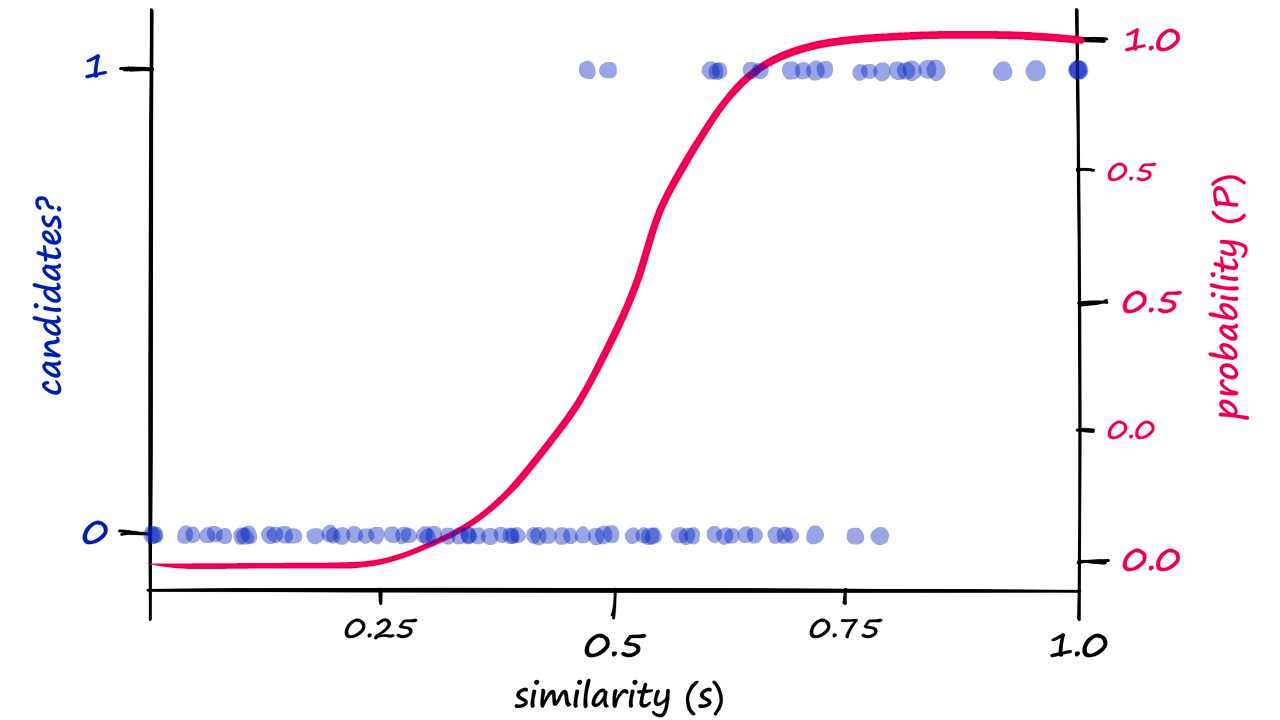
\includegraphics[width=\textwidth]{lsh_threshold_curve.png}
\caption{固定参数时，LSH 会把相似度映射成一条近似阈值曲线。}
\end{subfigure}
\begin{subfigure}{0.48\textwidth}
\centering
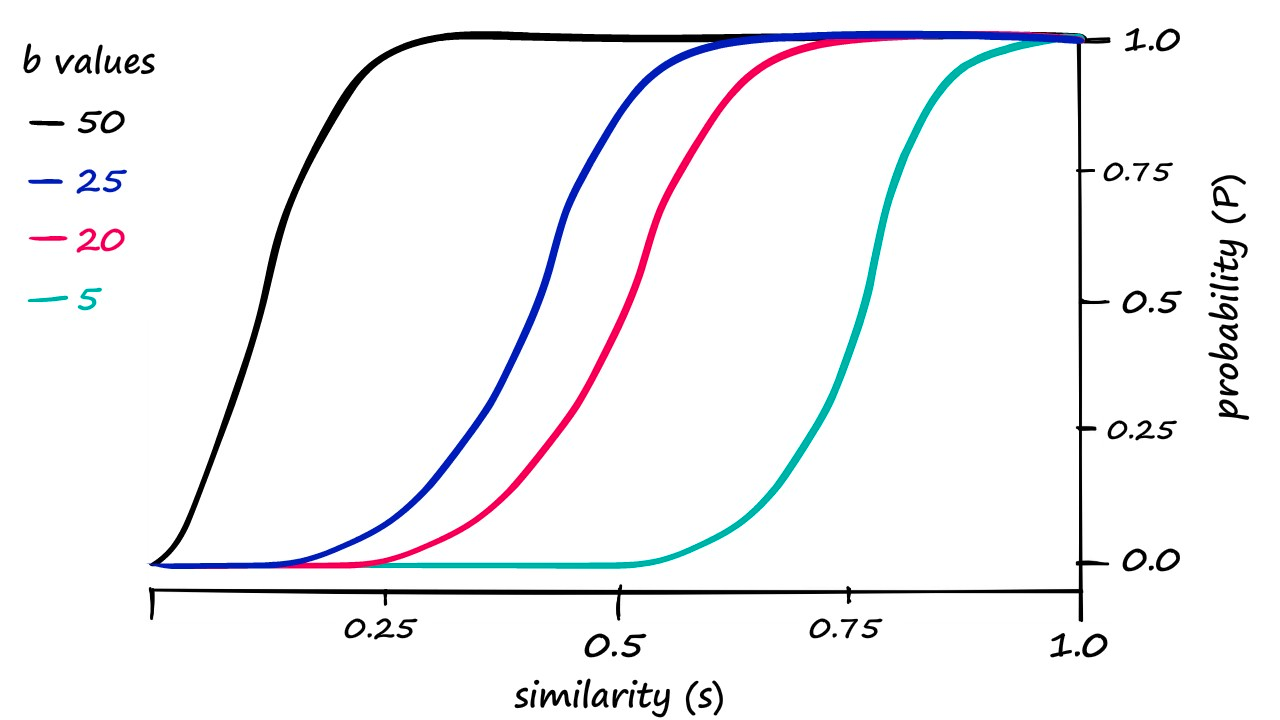
\includegraphics[width=\textwidth]{lsh_bands_curve.png}
\caption{改变 band 数 $b$ 会直接改变阈值位置和曲线陡峭程度。}
\end{subfigure}
\caption{LSH 的本质不是“更复杂的哈希”，而是用 band 参数把候选提名概率压成更像阈值函数的选择器。}
\end{figure}

这一步的工程意义很大。你不是在问“两个文档是否完全一样”，而是在问“我愿意把多高相似度的样本当成候选近重复”。LSH 的参数调优，本质上就是在把这个容忍度编码进算法。

\subsection{本章小结}
去重部分真正教会学生的是：大规模数据工程几乎所有算法都要围绕“线性规模可运行”来设计。Bloom filter、MinHash 和 LSH 之所以重要，不是因为它们优雅，而是因为它们让近重复检测在现实语料上可做。

\section{总结与延伸}
第 14 讲把数据工程的机械细节真正摊开了。

第一，\textbf{很多数据问题都能抽象成“从 raw pool 中选出更像 target 的子集”。} 这个统一视角把质量过滤、语言识别和主题筛选连接了起来。

第二，\textbf{KenLM/CCNet 代表了高速粗筛。} 简单语言模型虽然不够精细，但在超大语料上极具性价比。

第三，\textbf{fastText 和 DSIR 把过滤推进成学习式选择。} 一个偏分类，一个偏分布重加权，都是现代数据 pipeline 的常用武器。

第四，\textbf{同样的 machinery 可以服务不同目标。} 语言、质量、毒性、数学文本等都可以视作 target-definition 问题。

第五，\textbf{去重是算力效率问题，也是记忆化风险问题。} exact hash、Bloom filter、MinHash 和 LSH 一起构成了现实可扩展的去重工具箱。

\begin{warningbox}{我对第 14 讲的压缩提醒}
如果只记住“要做过滤、要做去重”，那还远远不够。真正要学到的是：\textbf{数据工程的核心挑战不是提出一个很聪明的定义，而是用足够便宜、足够可扩展的算法把这个定义在海量语料上真正跑起来。}
\end{warningbox}

到这里，CS336 的数据章节形成了闭环：第 13 讲讲全景和来源，第 14 讲讲算法和机制。接下来进入对齐章节时，你会发现后训练数据集的构建，同样遵守这里建立的“目标定义、过滤、去重和高价值保留”逻辑。

%% --- 正文内容结束 --- %%

\end{document}
